\documentclass[a4paper]{article}

\usepackage[french]{babel}
\usepackage[T1]{fontenc}
\usepackage[utf8]{inputenc}
\usepackage{float}
\usepackage{amsmath}
\usepackage{graphicx}
\usepackage{wrapfig}
\usepackage{lscape}
\usepackage{rotating}
\usepackage{epstopdf}
\usepackage{gensymb}
\usepackage{multirow}
\usepackage{lmodern}
\usepackage[left=3cm, right=3cm, bottom=4cm, top=4cm]{geometry}
\usepackage{array}
\usepackage{pdfpages}

\usepackage[gen]{eurosym}
\DeclareUnicodeCharacter{20AC}{\euro{}}

\usepackage{hyperref}
\hypersetup{
    colorlinks,
    citecolor=black,
    filecolor=black,
    linkcolor=black,
    urlcolor=black
}

\title{Rapport de pré-étude}

\author
{
	François {\sc Boschet}\\
    Arnaud {\sc Lods}\\
    Marlène {\sc Tuekam}\\
    Alexandre {\sc Bouchet}\\
    Guillaume {\sc Perrudin}\\
    Nguyen {\sc Song Hai}\\
    Romain {\sc Colombat}
}

\date{\today}

\newcommand{\pagevierge}[0]{\newpage\thispagestyle{empty}\null\newpage}

% Note
% Organisation pas bien - bien - tres bien
% Qualite contenu 
% Qualite mise en page
% Commentaires


\begin{document}
    % Ouh c'est sale.
    \hypersetup{pageanchor=false}
    
\includepdf[pages=1]{figure/couv.pdf}
    \hypersetup{pageanchor=true}

    \newpage
    \thispagestyle{empty}
    \mbox{}

    \newpage
    % A decommenter pour la release
    \setcounter{tocdepth}{2}
    \tableofcontents
    \setlength{\parskip}{10pt}

    \newpage
    \thispagestyle{empty}
    \mbox{}

    \newpage
    \section{Introduction}

    \section{Les Objectifs}
	\label{sec:objectifs}

    Le projet se résume donc à la réalisation d’une plateforme qui permettra aux utilisateurs
    de consulter des informations mais aussi d’interagir avec les éléments de l’application.
    En effet, si la tâche principale est de pouvoir accéder aux divers documents numérisés afin
    de consulter ceux-ci, l’utilisateur doit pouvoir accéder à d’autres fonctionnalités.
    Ainsi il serait possible de pouvoir apporter des modifications sur certaines annotations
    extraites des images numérisées sur divers documents pour apporter des informations
    supplémentaires sur ceux-ci ou en corriger certaines, mais il sera aussi nécessaire
    de permettre la création et la gestion de parcours thématiques par les utilisateurs
    afin d’offrir une navigation collaborative dans la presse ancienne.

    On peut donc résumer les objectifs de l’application de façon très concise :

    \begin{itemize}
        \item{Accéder aux documents numérisés}
        \item{Recherche à travers les documents}
        \item{Gestion des annotations de chaque document}
        \item{Création et gestion de parcours thématiques}
    \end{itemize}

    L’objectif principal est de gérer les données de milliers puis de millions de documents
    qui sont – et seront – numérisés et mis à disposition à travers la plateforme.
    Si au départ celle-ci ne contiendra que quelques milliers de documents, la base de données
    qui sera utilisée devra toujours être accessible rapidement afin de limiter les temps d’attente;
    au final un des objectifs importants sera d’optimiser la base de donnée reliée à l’application.

    Bien évidemment, la recherche d’éléments constitue la fonctionnalité clé de l’application,
    puisqu’il est primordial de pouvoir chercher et/ou retrouver efficacement un document
    en possédant certaines informations ou en ayant un domaine de recherche. Il sera donc nécessaire
    de proposer des champs de recherche pouvant couvrir tous les besoins, mais que celle-ci
    se fasse aussi assez rapidement. La recherche plein texte dans un document ou sur une page
    sera aussi important afin d’avoir un visuel direct sur des éléments que l’on pourrait rechercher
    dans une page, d’autant plus que certains journaux ont une résolution de 5000x4000 pixels et
    qu’il serait trop embêtant pour l’utilisateur de devoir chercher l’information de lui-même dans la page.

    Le but de pouvoir gérer les annotations, qui seront en partie initialisées après la récupération
    des informations du document, sera de permettre aux utilisateurs de corriger les données quand
    le résultat de l’analyse ne semble pas très pertinent, ou de rajouter des commentaires ou
    de nouvelles informations afin de fournir le maximum d’informations possibles et utiles aux utilisateurs.

    Enfin, dernier objectif mais pas des moindre, sera donc la gestion de parcours thématiques,
    créés par et pour les utilisateurs, afin de rassembler autour d’un même évènement,
    d’un même journal ou d’une même personnalité divers articles sélectionnés par ces mêmes utilisateurs
    afin de proposer, entre autres, des pistes de lecture. Le défi ici est de proposer de manière simple,
    automatique et pratique la création, la modification et le partage de ces parcours afin que cela
    ne devienne pas une besogne ceux qui souhaitent partager de l’information.


    \section{Les cibles}
\label{sec:cibles}
    L’application vise ici la totalité des utilisateurs qui pourraient être intéressés
    pour accéder à la presse ancienne numérisée. On a donc un public potentiel de toute provenance,
    des sciences humaines aux sciences techniques, qui trouverait de l’utilité à découvrir
    d’anciens articles sur des thématiques particulières. On peut aussi imaginer des personnes
    de tout âge cherchant à utiliser la plateforme : il n’est pas invraisemblable de trouver un intérêt
    à la création de parcours thématiques pour des exposés scolaires, et on peut donc
    se retrouver avec des utilisateurs très jeunes qui accéderaient à la plateforme, mais aussi
    des personnes plus âgées, qui ont moins de facilité et d’affinité avec les technologies récentes,
    qui pourraient vouloir accéder à cette information.

    Il faut donc prendre en compte que l’on va avoir une base d’utilisateur très large,
    et que l’utilisation de la plateforme doit être la plus simple et intuitive possible
    afin que ceux-ci ne soient pas perdus ou découragés. De plus, une base d’utilisateurs
    venant de divers horizons signifie aussi des utilisateurs souhaitant accéder à l’application
    à travers diverses plateformes ; il ne sera pas étrange de retrouver des utilisateurs sous Windows
    comme sous Mac, Android, Linux… il sera donc nécessaire d’avoir une plateforme compatible
    sur n’importe quel distribution, pouvant s’adapter à n’importe quel format (PC, tablette mais aussi smartphone).


    \section{État de l'art}
\label{sec:etat_art}

    \subsection{Numérisation de documents}
    \label{subsec:numerisation}
    Même si le sujet se centre sur la consultation de documents numérisés, il est intéressant de remarquer qu’il existe plusieurs
    solutions aujourd’hui pour pouvoir numériser des documents anciens. En effet un nombre non négligeable d’entreprises proposent
    aujourd’hui la numérisation de nombreux types de documents, ce qui signifie qu’il y a aussi une certaine demandes non négligeable
    et un besoin de pouvoir accéder à de vieux documents de nouvelles manières.


        \subsubsection{Arkhenum}
        \label{subsubsec:arkhenum}

        Arkhenum est une entreprise spécialisée dans la numérisation de documents anciens
        datant du Vème au XXème siècle. Les types de documents numérisés sont très variés :
        cartes, plans, archives (registres d'état civil, paroissiaux, militaires, etc),
        affiches, livres, manuscrits, etc. Arkhenum travaille à la demande de bibliotèques,
        de centres d'archives, de cinématèques ou bien de musées. L'idée est d'utiliser
        la numérisation afin de préserver et de diffuser ces documents.

        La valeur d'Arkhénum est avant tout la préservation des documents, un soin particulier
        est donc apporté à la manipulation des documents, le protocole de numérisation
        est donc adapté : pas de vitre de numérisation, ouverture des reliures limitée à 120\degree,
        utilisation de gants en coton. Arkhénum mise également sur la haute qualité
        des numérisations en adaptant l'éclairage, le cadrage et en appliquant des traitements
        de correction des courbures.

        Arkhenum se pose en tant que service de numérisation plutôt que plateforme de diffusion.
        C’est le client à l’origine de la numérisation qui se charge de la diffusion
        des documents numérisés. L'activité de notre projet se situe donc à posteriori de l'activité d'Arkhénum.


        \subsubsection{Azentis}
        \label{subsubsec:azentis}
        Azentis a une activité beaucoup plus large. C’est une entreprise travaillant sur la totalité du processus de conservation
        de documents, de la  numérisation à la diffusion. Les documents numérisés sont de types variés : archives (registres d'état civil,
        paroissiaux, parchemins, livres anciens, livres, presse ancienne, cadastres), documents (techniques, commerciaux, personnels,
        comptables, logistiques, d'urbanisme, etc), photos, plans.

        Azentis est également présent sur la diffusion. En effet, elle développe des solutions de consultation de documents numérisés
        ayant des fonctions de recherches par mot clé. Cependant, ces solutions de consultation sont développées au cas par cas,
        pour chacun de ses clients. Il n'y a pas de plateforme publique de centralisation des documents numérisés.

    \subsection{Consultation de documents}
    \label{subsec:consultation}
    Il n’existe pas de plateforme dédiée qui référence et permette d’accéder à des documents de la presse ancienne. Cependant
    on peut constater de plus en plus un gain d’intérêt (notamment suite à des évènements comme les 100 ans de la Grande Guerre)
    d’accéder à des documents anciens qui peuvent être des actes de naissance, des registres d’état civil, des registres matricules ...
    et plusieurs plateformes ont vu le jour ces dernières années, permettant de consulter des documents de ce genre.


        \subsubsection{Archives des Yvelines}
        \label{subsubsec:yvelines}
        Archives Yvelines” est une plate-forme d’archivage et de consultation de documents antérieures
        à 1790 concernant les communes d’Yvelines, rassemblées pendant la Révolution. La plate-forme comporte
        près de 2 167 410 pages parmi lesquels des archives publiques et privées, ouvrages de bibliothèques,
        titres de presse locale, photographies et cartes postales, maquettes, pages numérisées,
        documents communiqués en salle de lecture, expositions virtuelles...

        La plate-forme des archives d’Yvelines permet de faire une recherche plus ou moins affinée
        en fonction d’une thématique (registres paroissiaux, recensement de population, répertoires
        de notaires, presse ancienne,. . . ) ou de la commune. Par exemple, pour une recherche dans
        les registres paroissiaux et d’état civil (illustrée par la figure ci contre), il est possible
        de choisir plusieurs critères d’affinement de la recherche comme la cote, le type d’acte, la période...
        La recherche par commune donne accès à tous les différents documents d’une commune.

        \begin{figure}[ht!]
            \centering
            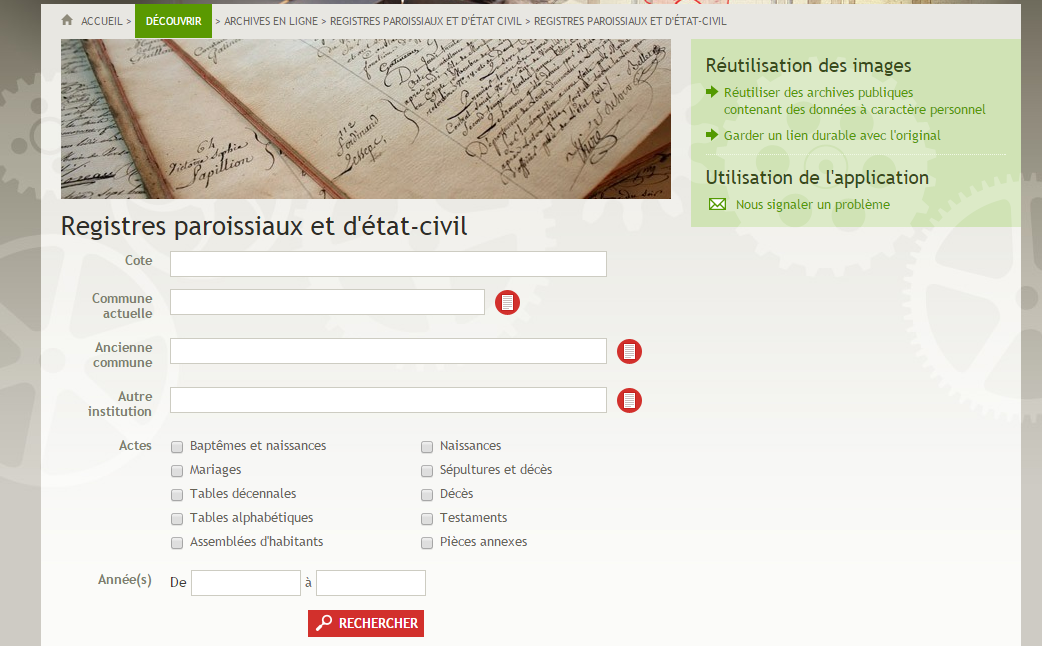
\includegraphics[width=1\textwidth]{figure/screen_yvelines_recherche.png}
            \caption{Capture d'écran de la recherche sur Archives Yvelines}
            \label{fig:yvelines_recherche}
        \end{figure}


        Après accès au document, il est possible d’effectuer plusieurs actions en fonction du type de document.
        Par exemple pour les documents numérisés, les principales actions sur le document sont le zoom,
        le téléchargement, la récupération du lien, l’ajout dans un panier, le signalement d’une erreur,
        l’annotation et l’impression (confère la figure ci-dessous).

        Il existe certains documents comme les fiches concernant les navires de guerre où il n’est possible
        d’effectuer aucune action pendant la consultation.

        \begin{figure}[ht!]
            \centering
            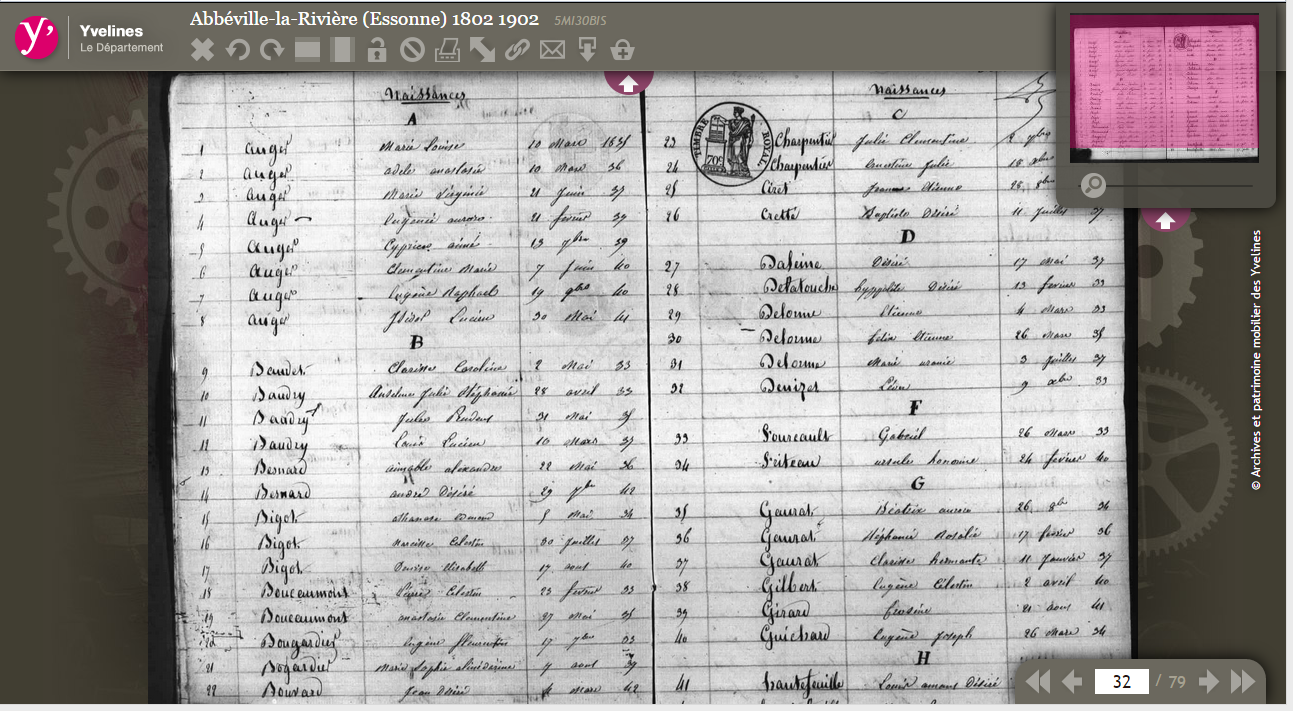
\includegraphics[width=1\textwidth]{figure/screen_yvelines_document.png}
            \caption{Capture d'écran de l'outil de visualisation d'un document sur Archives Yvelines}
            \label{fig:yvelines_doc}
        \end{figure}

        Concernant la consultation de presse ancienne (qui est l’objectif de notre projet),
        Archives Yvelines propose en plus de toutes les actions énumérées plus haut, une recherche
        en plein texte dans les journaux. La plate-forme propose aussi une annotation colaborative
        pour permettre des recherches par indexation dans la presse ancienne. Le service d’annotation
        n’est disponible que pour les utilisateurs possédant un compte; ce qui peut être assez contraignant
        pour certains utilisateurs

        \subsubsection{Mémoire des hommes}
        \label{subsubsec:memoire}
        Mémoire des hommes” est aussi une plate-forme de consultation d’anciens documents
        et qui a été inaugurée en 2003. Elle comporte essentiellement des fiches numérisées concernant
        les militaires français acteurs des conflits tels que la première et seconde guerre mondiale,
        la guerre d’Indochine, la guerre de Corée, ou encore la guerre d’Algérie.

        Le site “Mémoire des hommes” permet d’effectuer une recherche soit grâce aux indexations
        réalisées à l’aide des annotations des utilisateurs, soit par thématique de guerre.
        Il est possible d’affiner la recherche avec des informations concernant la personne telles que le nom,
        la date de naissance, le lieu de naissance, le département, ...

        Les actions réalisables sur les documents sont identiques à celles de la plate-forme
        des archives d’Yvelines, les deux plate-formes utilisant le même outil pour la visualisation
        de documents.

        Le site ‘Mémoire des hommes’ possède une petite particularité qui est la cartographie pour
        certaines guerre comme la guerre de Corée ; cartographie sur laquelle et localisée chacune
        des batailles de la guerre, la période et le nombre de décès.

        \begin{figure}[ht!]
            \centering
            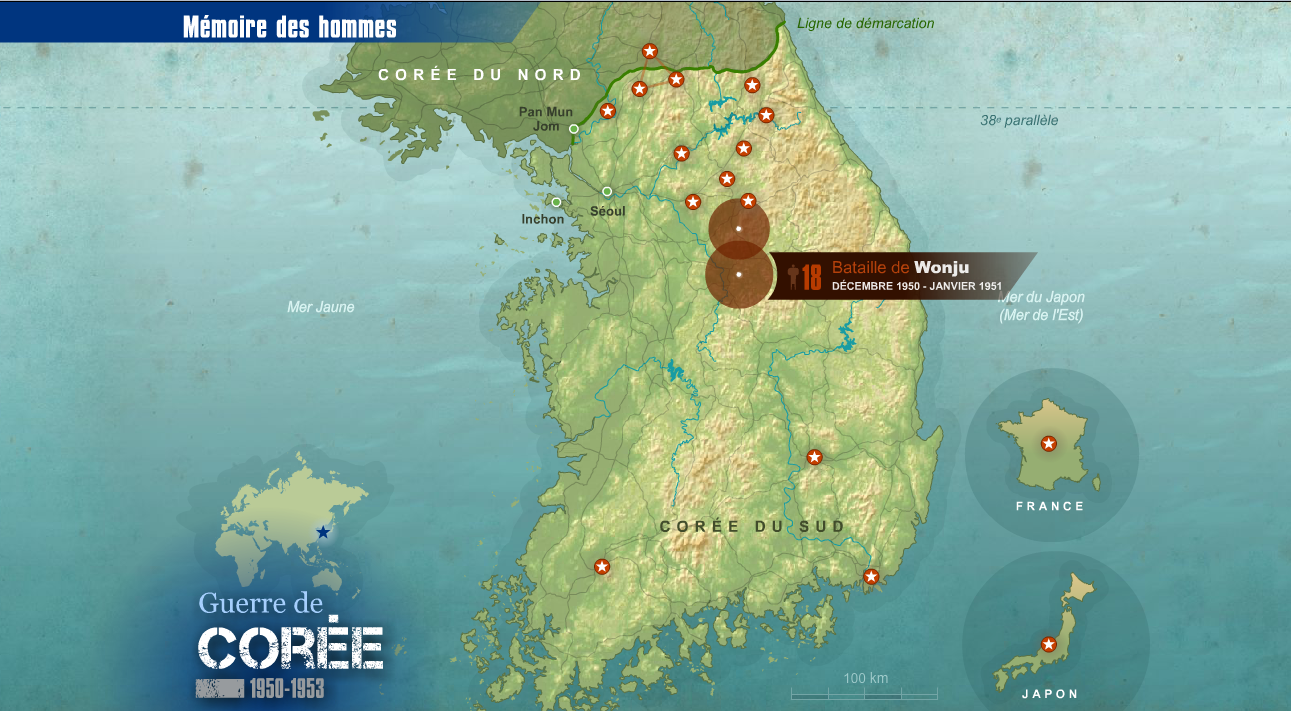
\includegraphics[width=1\textwidth]{figure/screen_memoire_hommes.png}
            \caption{Capture d'écran de la cartographie Mémoire des hommes}
            \label{fig:memoire_hommes}
        \end{figure}

        \subsubsection{Numdam}
        \label{subsubsec:numdam}
        C’est un programme de la Cellule de coordination documentaire nationale pour les mathématiques (Mathdoc) soutenant des revues
        de mathématiques en rendant leurs archives consultable sur internet. Les revues sont scannées en haut définition et mises
        à disposition en format djvu ou pdf. Le texte des pdfs est protégé contre la copie mais on peut cependant faire
        une recherche de mots dessus. On note la présence du format djvu adapté aux liseuses électroniques, ce dernier n’est
        pas protégé contre la copie du texte. La bibliothèque est relativement “pauvre” avec une collection de 36 journaux, 32 séminaires et 5 mémoires.

        \subsubsection{Gallica}
        \label{subsubsec:gallica}
        C’est la bibliothèque numérique de la Bibliothèque nationale de France, elle est en ligne depuis 1997.
        La bibliothèque est très riche de contenu avec aujourd’hui plusieurs millions de documents
        et chaque semaine des milliers de nouveautés. On peut consulter les œuvres directement sur le site,
        nous avons accès à tout un panel de commandes pour naviguer dans l’ouvrage: flèches suivant/précèdent,
        zoom, rotation, plein écran, recherche sur le texte, mode d’affichage, téléchargement, partage,
        signaler une anomalie. On a accès à des légendes en rapport avec l’œuvre et dans le même panel
        au texte où l’on peut effectuer une recherche plein texte. Cependant, le texte, reconnu avec un OCR
        (Optical character recognition - Reconnaissance optique de caractère), est parfois inexact.
        Gallica informe avoir eu recourt à deux types d’OCR, un OCR brut sans intervention humaine ou un OCR
        avec montée en qualité du texte ou celui-ci est amélioré par une correction manuel. On peut ainsi
        attendre un taux qualité cible de 96 à 99.9\% avec l’OCR le plus qualitatif. 

        \begin{figure}[ht!]
            \centering
            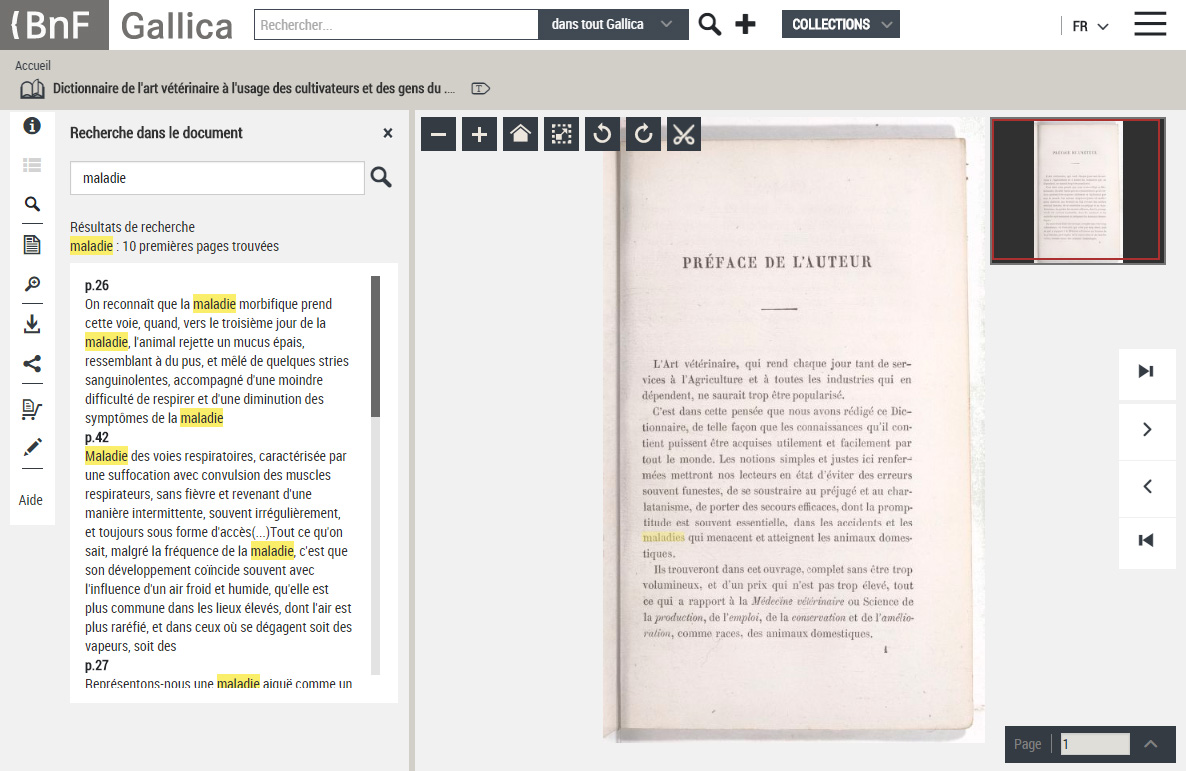
\includegraphics[width=1\textwidth]{figure/screenshot_gallica.jpg}
            \caption{Capture d'écran du moteur de recherche Gallica}
            \label{fig:gallica}
        \end{figure}

        Pour le téléchargement, on peut télécharger le document en entier ou une sélection du document soit en pdf,
        soit en jpeg pour la page en cours. Les options de consultation évoluent aussi en fonction du type de texte,
        ainsi la légende, recherche dans le document ou table des matières ne sont pas disponible pour tous les ouvrages.
        Pour les manuscrits par exemple on n’aura accès au texte plein et pour les revues souvent juste la table des matières.
        Outre la visionneuse disponible sur le site web, Gallica propose des applications mobiles sur Google Play et App Store.
        Bien que le site de Gallica soit responsive, l'existence d’application mobiles qui imite le site est intéressant.
        Le site ne propose qu’une navigation sommaire entre une série d’image lorsque l’ont se rend sur celui ci depuis un navigateur pour mobile.

        En ce qui concerne la section presse et revues du site plus particulièrement, la visionneuse ne propose
        pas d’options spécifiques à ce type de document. Sur la plus part des revues nous n’avons pas accès à l’OCR
        c’est pourquoi il serait intéressant d’implémenter cette fonctionnalité pour notre projet.

        \subsubsection{archives.morbihan}
        \label{subsubsec:morbihan}
        Ce site concerne les archives du Morbihan. L’ outils de consultation de presse ancienne est presque semblable
        (en termes de services offerts) à celui proposé par les archives d’Yvelines. Le site propose une application
        de filtres sur les documents (comme l’illustre la figure ci-dessous). Il propose aussi une version texte des
        articles de journaux. Cependant il n’est pas possible d’effectuer une recherche sur la version texte,
        ce qui est assez utile et pratique.

        \subsubsection{britishnewspaperarchive}
        \label{subsubsec:britishnewspaper}
        La plate-forme “britishnewspaperarchive” est un site de consultation de presse ancienne du Royaume Uni.
        Le site comporte près de 12 millions de pages de journaux allant de 1710 à 1959. Il est possible
        d’effectuer une recherche par période, région, pays, ville, ou encore par journal. La consultation
        des journaux est cependant payante à hauteur de £12,95 le mois, ce qui est une véritable contrainte
        pour un utilisateur non régulier.

        \subsubsection{archive.winnipegfreepress}
        \label{subsubsec:winnipeg}
        C’est un site américain de consultation de presse ancienne qui permet d’effectuer une recherche par période,
        thématique, ou mots clés. La consultation des journaux ici  est aussi payante
        (\$9,18/semaine) . Mais le site propose une période d’essai gratuite de 14 jours donnant accès à tous les documents de presse.

        \subsubsection{Chronicling America}
        \label{subsubsec:chrinamerica}
        “Chroniclingamerica” est une plate-forme de consultation de presse ancienne américaine qui offre des services
        tels que le zoom, le rognage, l’impression, le téléchargement sous forme d’image ou pdf. Le site propose
        aussi une consultation du journal sous forme de texte permettant ainsi de faire une recherche classique
        (à l’aide d’un Ctrl+F). Cependant la mise en forme de la version texte du journal ne facilite pas beaucoup la lecture.



    \section{Solutions techniques}
\label{sec:technique}

    \subsection{Type de la plateforme}
    \label{subsec:plateforme}
    Il n’y a aucune contrainte quant à la réalisation de la plateforme, si ce n’est qu’elle doit être accessible
    pour tous types d’utilisateurs : PC (Windows/Mac/Linux), Tablettes (Android/iOS) voir même Smartphones
    (Android/iOS/Windows phone/Blackberry…). Il serait envisageable d’imaginer réaliser une application multiplateforme
    qui puisse être installée et puisse fonctionner sur tous types de plateforme, cependant cela imposera
    de très nombreuses contraintes techniques, il faudra sans cesse penser à cette comptabilité et les tests
    n’en seraient que plus embêtant. Il est bien évidemment exclus de réaliser une application unique à chaque plateforme,
    ne serait-ce que pour le temps de développement mais aussi lors de la reprise de celle-ci dans le futur qui rendrait
    ceci très difficile.

    Il semble donc naturel de partir sur le développement d’une plateforme web, ce qui permettra de la rentre compatible
    avec n’importe quel navigateur et facilitera la communication client/serveur (qui aurait pu poser des problèmes
    si l’application installée sur la machine de l’utilisateur devait communiquer avec un serveur). De plus la gestion
    de comptabilité entre les différents formats de visualisation sera réalisée grâce aux outils de design que permet
    une application web, cela facilitera l’implémentation.

    \subsection{Technologie de la platefome}
    \label{subsec:technologie}
    Il existe plusieurs langages qui permettraient de développer une application web comme celle-ci.
    Chaque langage a ses propres avantages et inconvénients, nous allons ici présenter de façon exhaustive
    chaque langage possible avant de lister les avantages et inconvénients de chacun. Ces choix feront lieu
    d’un débat lors d’une réunion du groupe afin de décider d’une technologie à utiliser pour commencer
    à la prendre en main et réaliser une ébauche afin de voir ce que l’on sera capable de faire de nous-même
    avec, et ce avant le développement de la plateforme.


        \subsubsection{PHP}
        \label{subsubsec:php}
        PHP est utilisé sur plus de 75\% des serveurs web ; il y a plus de 27 millions de sites web qui
        sont codés en PHP, ce qui correspond à 50\% des sites web dans le monde. C’est un langage
        polyvalent et il est considéré comme le langage web standard. Ce langage est notamment privilégié
        car il est simple à apprendre et il est très simple d’installer un serveur web fonctionnant sous PHP,
        que ce soit sous Windows, Max ou Linux. Il est aussi à l’origine de quelques plateformes comme
        WordPress, Wikipedia, et est même utilisé dans une partie de Facebook. PHP a été imaginé pour
        créer des sites webs. 

        De plus de très nombreux frameworks imaginés pour le développement de sites web existent
        et fournissent des outils spécifiques permettant d’améliorer l’efficacité du code. La bibliothèque de
        PHP est aussi bien riche et diversifiée ; ce qui nous permet de résoudre presque tous les problèmes
        qui peuvent arriver en réalisant un site web.

        \subsubsection{Node.js / Javascript}
        \label{subsubsec:node}
        A ne pas confondre avec Java, Javascript est un “maître” qui nous permet de faire des
        interactions dans notre site web. C’est un langage particulier qui fonctionne en fonction de la
        navigation de l’utilisateur. Il nous permet d’interagir avec le site web avec des évènements et permet
        de mettre à jour dynamiquement des éléments sans avoir à recharger une page. Pour ce projet,
        l’utilisateur interagira avec divers éléments très souvent et il serait très embêtant pour lui de devoir
        attendre le rechargement de pages. Le langage propose notamment un framework très connu,
        JQuery, qui permet d’écrire beaucoup moins de code tout en améliorant l’interactivité de la
        plateforme.

        Node.js est une technologie très récente, encore jeune, permet tout simplement de gérer un
        serveur entièrement en Javascript. En effet il était de base nécessaire de manipuler PHP côté serveur
        et Javascript côté client. On a ici l’avantage de gérer ces deux parties dans un seul langage, ce qui
        facilite énormément la reprise d’un projet. De plus, Node.js montre aussi de très bonnes
        performances qui restent stables quel que soit le nombre d’utilisations, il faut cependant avec une
        très bonne connaissance de Javascript pour gérer le serveur par cette technologie.

        \subsubsection{Ruby}
        \label{subsubsec:ruby}
        Ruby est accompagné d’un framework, Ruby on Rails, pour developper un site. Il est
        fortement utilisé dans quelques grands sites web comme Groupon, Shopify, … et est utilisé pour faire
        le front-end du site web social Twitter. Ruby est open-source, c’est un langage orienté objet et est
        interprété par le serveur avant d’envoyer du code HTML au navigateur de l’utilisateur (comme PHP).

        Pourtant, Ruby a ses points forts: développement des applications très rapides, moins de répétition
        de code et le temps de traitement est plus court que PHP. Ruby on Rails a été imaginé pour faire des
        sites web compliqués, et comme Perl, plus performant. Néanmoins, Ruby a aussi un point faible ;
        contrairement à PHP il existe un moins grand nombre de serveurs qui supportent Ruby par défaut.

        \subsubsection{Python}
        \label{subsubsec:python}
        Python est un langage orienté objet, open-source ; c’est aussi un langage très facile à apprendre
        et qui possède une syntaxe simple à relire. Python est un bon outil pour programmer mais il n’est
        pas très utilisé en programmation site web. Pourtant Python est un bon choix pour les débutants et
        surtout pour les gens qui veulent faire des projets Linux ou pour une communauté open-source.

        \subsubsection{.NET}
        \label{subsubsec:dotnet}
        .NET ou ASP.net est un produit de Microsoft qui vise à concurrencer les autres technologies web.
        Cette plateforme est bien utilisée dans les entreprises mais un nombre restreint de site web
        sont actuellement développés avec ce langage, notamment car il n’est compatible que sur Microsoft Server.
        De plus, l’apprentissage de .Net est difficile, et il existe moins d’experts de cette technologie,
        ce qui est un élément important à prendre en compte pour la reprise éventuelle du développement de la plateforme.



        \subsubsection{Récapitulatif}
        \label{recap}
        \begin{tabular}{|l|l|}
            \hline
            Solution & Qualités/Défauts \\ \hline
            \multirow{8}{*}{PHP} & + Fonctionne sur tous les serveurs acceptant PHP (presque tous) \\
                & + Pas besoin de différencier les navigateurs du marché \\
                & + Langage web le plus répandu et le plus utilisé \\
                & + De nombreux frameworks disponibles \\
                & - Nombreuses failles de sécurité \\
                & - Langage interprété problème de performances si beaucoup de clients \\
                & - Non typé \\
                & - Débogage difficile \\ \hline
            \multirow{5}{*}{Node.js} & + Très performant, mëme si de nombreuses utilisations \\
                & + Temps de traitement et de changement faibles \\
                & + Communauté très active \\
                & - Nécessite une bonne maîtrise du langage Javascript \\
                & - Technologie jeune, pas de preuves de durée sur le long terme \\ \hline
            \multirow{6}{*}{Ruby} & + Langage concis, code plus lisible et reprise plus aisée \\
                & + Langage fortement orienté objet \\
                & + Gestion de librairie avec Bundler \\
                & + Communauté très active \\
                & + Framework Ruby on Rails \\
                & - Langage interpreté: problème de performances si beaucoup de clients \\ \hline
            \multirow{6}{*}{Python} & + Syntaxe simple et facilement lisible \\
                & + Nombreuses bibliothèques disponibles \\
                & + Communauté énorme et active \\
                & + Permet d’intégrer un code écrit dans un autre langage \\
                & - Détection d’erreur à l’exécution \\
                & - Langage interprété : problème de performances si beaucoup de clients \\ \hline
            \multirow{6}{*}{.Net} & + Langage compilé, éxecution plus rapide \\
                & + Possibilité d'utiliser plusieurs langages \\
                & + Garbage collector \\
                & - Ne fonctionne que sur Microsoft Server \\
                & - IDE très lourd \\ 
            \hline
        \end{tabular}

    \subsection{Gestion de la base de données}
    \label{subsec:bdd}

   Notre plateforme disposera aussi d’une base de données afin de stocker les données des documents numérisés
   ainsi que celle des comptes utilisateurs. Il est nécessaire de distinguer deux types de système de gestion de base de données.

    D’un côté, les bases de données relationnelles. Ce sont des bases où les données sont organisées
    sous forme de tables (ou relation) à deux dimensions. C’est le système de base de données le plus utilisé.
    Les bases de données sont manipulées à l’aide du langage SQL. La présence d’un schéma relationnel qui structure
    les données permet de faire des requêtes riches, ce qui permet de manipuler efficacement les données.

    D’un autre côté, le NoSQL, qui comprend tous les systèmes de base de données qui ne se basent pas sur une
    architecture relationnelle. Le but est de gagner en simplicité, notamment en s’affranchissant du schéma relationnel
    qui est fixé lors de la création de la table, et qui contraint l’ajout de nouvelles données. Un exemple de modèle en NoSQL,
    c’est un système de clé-valeur. La base de données peut se résumer alors à un tableau associatif avec des millions d’entrées.
    Cependant, cette simplicité réduit la richesse des requêtes et déplace la complexité intrinsèque de la requête vers
    la logique de l’application. En revanche, ce système de base de données gère mieux le cas où les données sont réparties
    sur plusieurs serveurs.

    \subsubsection{ElascticSearch}
    \label{subsubsec:elasticsearch}
    ElasticSearch est une base de données orientée sur la recherche.
    Elle propose des possibilités de recherche intelligente. En effet, il est par exemple possible
    d'effectuer des recherches mal orthographiées, ElasticSearch se charge alors de trouver des ressemblances
    entre les mots et propose alors des résultats avec un taux de confiance.

    ElasticSearch est accessible une API REST permettant d'effectuer des requêtes facilement.Elle est facilement scalable :
    la réplication des données au sein d'un cluster s'effectue en toute transparence.
    C'est donc une technologie qu'il serait intéressant d'utiliser dans le projet, pour permettre à l'utilisateur
    de d'effectuer des recherches d'articles efficacement.

    Dans la plupart des cas d'usages, elle n'est pas utilisée en base de données principale. En général,
    les modifications de données sont effectuées une base de données principale (PostgreSQL, MongoDB, etc);
    et les consultations/recherches de données sont effectuées sur ElasticSearch. Les données doivent donc être répliquées sur ElasticSearch.

    Cette séparation des tâches est intéressant d'un point de vue performance. En effet, en cas d'utilisation intensive
    des ressources du serveur, il serait tout a fait envisageable d'avoir une base de données principale sur un serveur,
    et ElasticSearch sur un autre.


        \subsubsection{Liste des solutions}
        \label{subsubsec:bddsolutions}

        \begin{center}
        \begin{tabular}{|l|l|l|}
            \hline Type & Solutions & Qualités/Défauts \\ \hline
            \multirow{20}{*}{SQL} & \multirow{4}{*}{Oracle} & + Très performant \\
            & & + Très bon temps de réponse \\
            & & + Fournis beaucoup d'outils \\
            & & - Licence propriétaire \\ \cline{2-3}
            & \multirow{4}{*}{MySQL} & + Gratuit \\
            & & + Très performant sur des petits volumes de données \\
            & & + Très performant avec un faible accès \\
            & & - Performance très faible sur des grosses bases de données \\ \cline{2-3}
            & \multirow{6}{*}{PostgreSQL} & + Communauté très active \\
            & & + Respecte la norme SQL2003 \\
            & & + Beaucoup d’outils disponibles \\
            & & + Gère très bien de gros volumes de données grâce à son optimiseur \\
            & & - Moins performant que d’autres sur des petits volumes de données \\
            & & - Nécessite une très bonne configuration et une base entretenue \\ \cline{2-3}
            & \multirow{6}{*}{Windows Access} & + Facile d’utilisation et de maintenance \\
            & & + Très rapide à mettre en œuvre \\
            & & - Licence propriétaire \\
            & & - N’est pas fait pour traiter beaucoup de données \\
            & & - Données stockées dans un fichier \\
            & & - Utilisation restreinte à Windows \\ \hline
            \multirow{15}{*}{NoSQL} & \multirow{5}{*}{MongoDB} & + Solution NoSQl la plus populaire \\
            & & + Permet de manipuler des objets structurés \\
            & & + Ne nécessite pas de schéma prédéfini des données \\
            & & - Ne respecte pas l’ensemble des propriétés A.C.I.D. \\
            & & - Difficilement scalable \\ \cline{2-3}
            & \multirow{4}{*}{Cassandra} & + Très performants pour des bases distribuées \\
            & & + Propriétés ACID respectée par ligne \\
            & & - Schéma défini à l’avance car système orienté colonne \\
            & & - Rigide lors de la recherche \\ \cline{2-3}
            & \multirow{6}{*}{Couchbase} & + Facilement scalable \\
            & & + Permet de manipuler des données déstructurées \\
            & & + Requêtage avec un langage proche du sql : N1QL \\
            & & + Avantage du monde relationnel et du monde NoSQL \\
            & & - Utilisé en production mais encore jeune \\
            \hline
        \end{tabular}
        \end{center}

    \subsection{Besoins de la plateforme}
    \label{subsec:besoinplateforme}
    Les caractéristiques mises en avant précédemment sont d’ordre général. Nous allons à présent
    regarder vis-à-vis des particularités de notre base de données.

    Les données que nous manipulerons seront nombreuses, l’application est destinée entre autres
    à des services d’archives départementales qui ont des dizaines de milliers de documents numérises
    et ce nombre s’accroit. Ce sont aussi des données plutôt volumineuses (plusieurs Mo le document).
    Cela signifie que nous avons besoin d’une solution qui soit optimisée pour ce genre de cas tout
    en restant performant car l’utilisateur ne doit pas attendre longtemps l’affichage du document.
    Donc, MySQL ne figure pas dans les meilleures solutions pour cette particularité.

    La solution devra aussi nous permettre d’implémenter le concept de document numérisé de manière
    à ne pas rendre le travail de manipulation des données trop complexe. De même, nous aurons besoin
    de faire des recherches en fonction du titre, de l’année… Le langage devra permettre cela.
    Cependant, nous pouvons accepter les langages qui ne proposent qu’une recherche rudimentaire
    car nous pourrons implémenter une recherche plus sophistiquée avec le langage de l’application.
    C’est le cas, par exemple, de MongoDB.

    Il faut prendre aussi une particularité intrinsèque au projet : la connaissance du langage.
    En effet, utiliser un langage que nous maitrisons déjà nous permettrait de gagner du temps.
    C’est le cas du SQL que nous avons vu lors de notre cursus scolaire. Cependant apprendre
    un nouveau langage est toujours un apport ludique. Les projets sont l’occasion d’utiliser
    des langages différents de ceux enseignés dans le cursus. Mais il ne faut pas non plus choisir
    un langage trop obscur car le projet sera probablement poursuivi les années suivantes.
    Il serait préférable que le langage choisi soit motivant pour les prochains groupes qui travailleront sur le projet.

    Enfin, certaines solutions sont des licences propriétaires. Cela signifie que l’utiliser nécessite
    d’acheter une licence. Nous aimerions éviter d’avoir à utiliser ce genre de solutions non seulement
    pour une raison financière mais aussi parce que nous préférerions  que notre plateforme soit open source.


    \section{Organisation du projet}
\label{sec:orga}

	Les différents délivrables du projet 4INFO imposent une gestion de projet suivant un modèle de cycle en V. Cependant, nous sommes libres d'adapter nos propre méthodes de développement 

	Ici, on a de nombreuses fonctionnalités que l'on va être amené à réaliser. Il est possible que l'on ne soit pas capable de toutes les réaliser; nos ressources étant limitées (3 développeurs) tout comme le temps disponible. Il est donc nécessaire de penser à une bonne méthode de gestion lors du développement. D'un côté, il est nécessaire d'évaluer l'importance de chaque fonctionnalité, définie bien précisément, et de l'autre, partie la plus alératoire, il nous faut estimer la durée de délivrable de celles-ci.

	En gardant un modèle de cycle en V, on se retrouverait donc à développer la plateforme, puis à effectuer différentes séries de tests avant de le délivrer. Le problème de cette méthode est que l'on va devoir faire une sélection de fonctionnalités à développer, s'y tenir, et un livrable ne sera fournit qu'à la fin. Entre autre, on ne pourra avoir un retour sur l'application lorsque le développement sera fini. Il sera impossible d'inférer sur les fonctionnalités puisqu'il n'y aura aucun retour durant le temps de développement. 

	C'est pourquoi nous pensons planifier le développement de l'application en se basant sur les méthodes agiles. On aura donc une liste de fonctionnalités, triées suivant leur importance et leur difficulté, à développer. En considérant les ressources mises à disposition, on délivrera et on effectuera en continue des tests pour chacun des fonctionnalités. Ainsi il sera possible de présenter l'avancement au milieu du projet à nos encadrant pour pouvoir adapter les fonctionnalités restantes, ou en rajouter par la suite. Si celles-ci se trouvent être plus intéressantes (plus intéressante/plus facile), on pourrait se retrouver à les développer avant des fonctionnalités définies avant. Enfin, cela permet à un instant T d'avoir un produit fonctionnel.

    \pagebreak


    % Manoucherie incoming
    \pagevierge
    \ifthenelse{\isodd{\thepage}}
    {\pagevierge}
    {}
    
\includepdf[pages=2]{figure/couv.pdf}
\end{document}
